\subsection{PolicyEngine Integration and Access}

The enhanced dataset is designed to integrate seamlessly with PolicyEngine, an open-source tax-benefit microsimulation platform available both as a Python package and a web application at \url{policyengine.org}. The platform provides comprehensive tools for analyzing tax and benefit reforms through both programmatic and web interfaces.

\subsubsection{Web Interface}

PolicyEngine's web interface at \url{policyengine.org/us} allows users to:
\begin{itemize}
    \item Modify thousands of policy parameters across federal and state tax and benefit programs
    \item Analyze reforms' impacts on:
    \begin{itemize}
        \item Government budgets (federal taxes, benefits, and state/local taxes)
        \item Income distribution (gains and losses across the income spectrum)
        \item Poverty (by age, race/ethnicity, and sex using the SPM)
        \item Inequality (various metrics)
        \item Labor supply (with customizable elasticities)
    \end{itemize}
    \item Generate natural language summaries of policy impacts using Claude 3.5 Sonnet
    \item Calculate household-specific impacts by entering detailed information
    \item View marginal tax rates under current law and reforms
\end{itemize}

\begin{figure}[h]
    \centering
    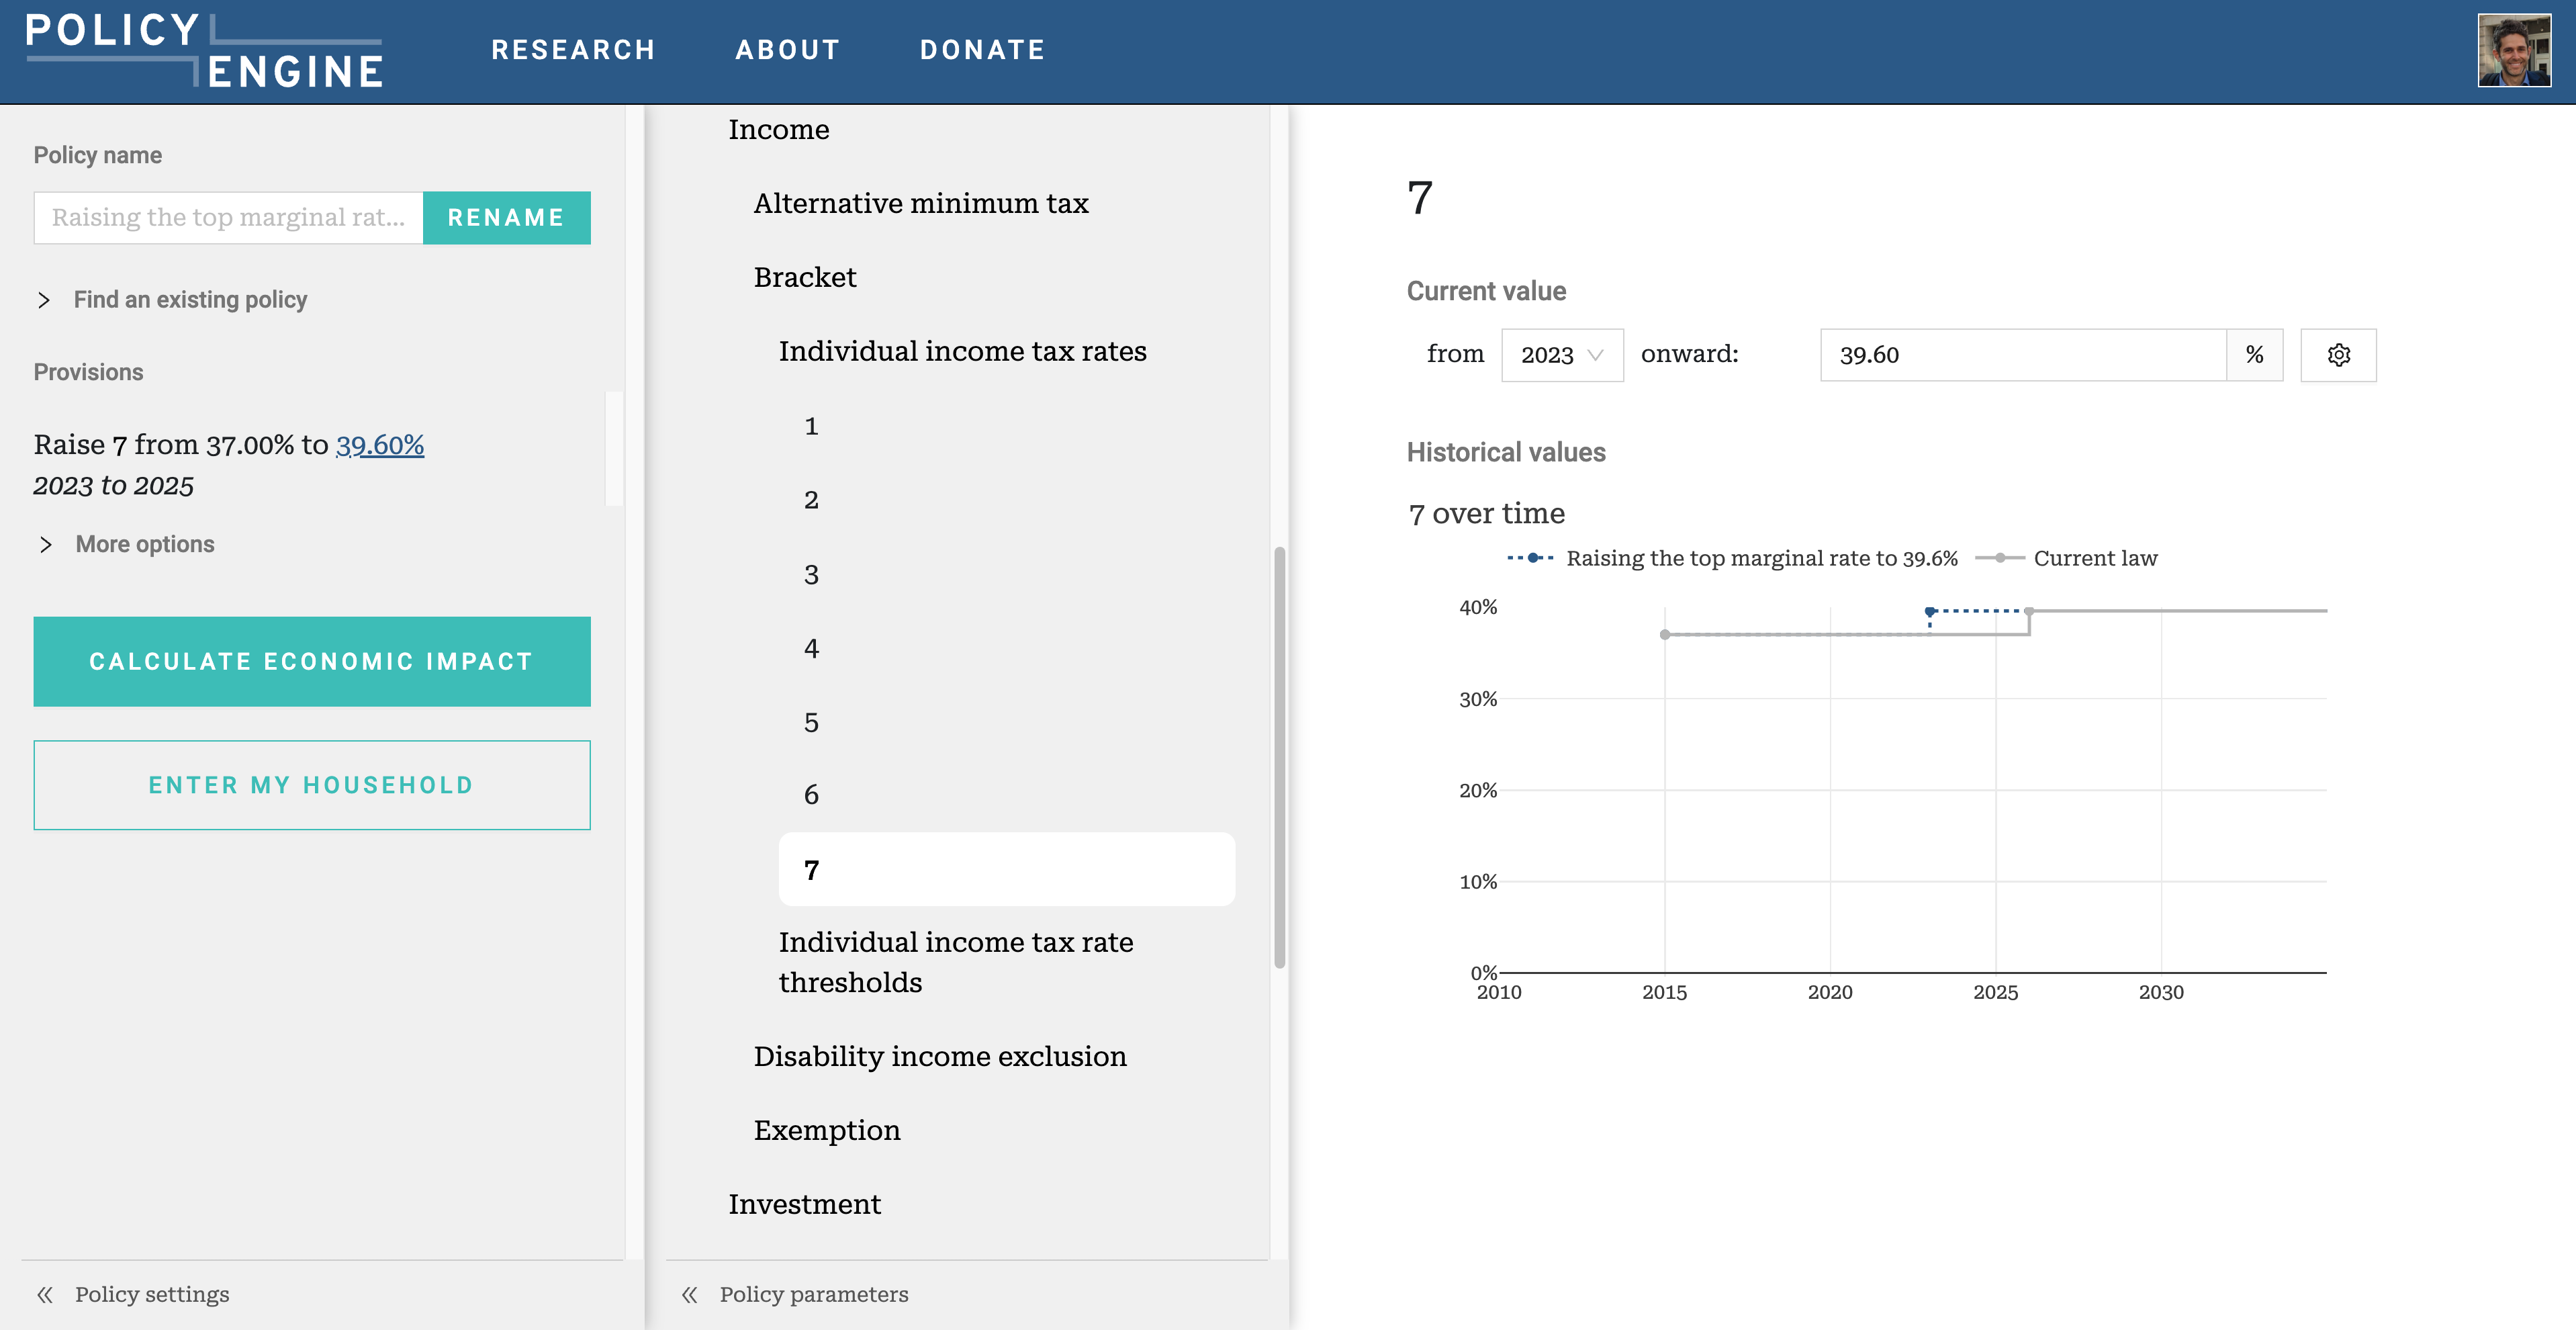
\includegraphics[width=\textwidth]{figures/policyengine_policy.png}
    \caption{PolicyEngine's policy editor interface, showing modification of the top marginal tax rate.}
    \label{fig:policyengine_policy}
\end{figure}

\begin{figure}[h]
    \centering
    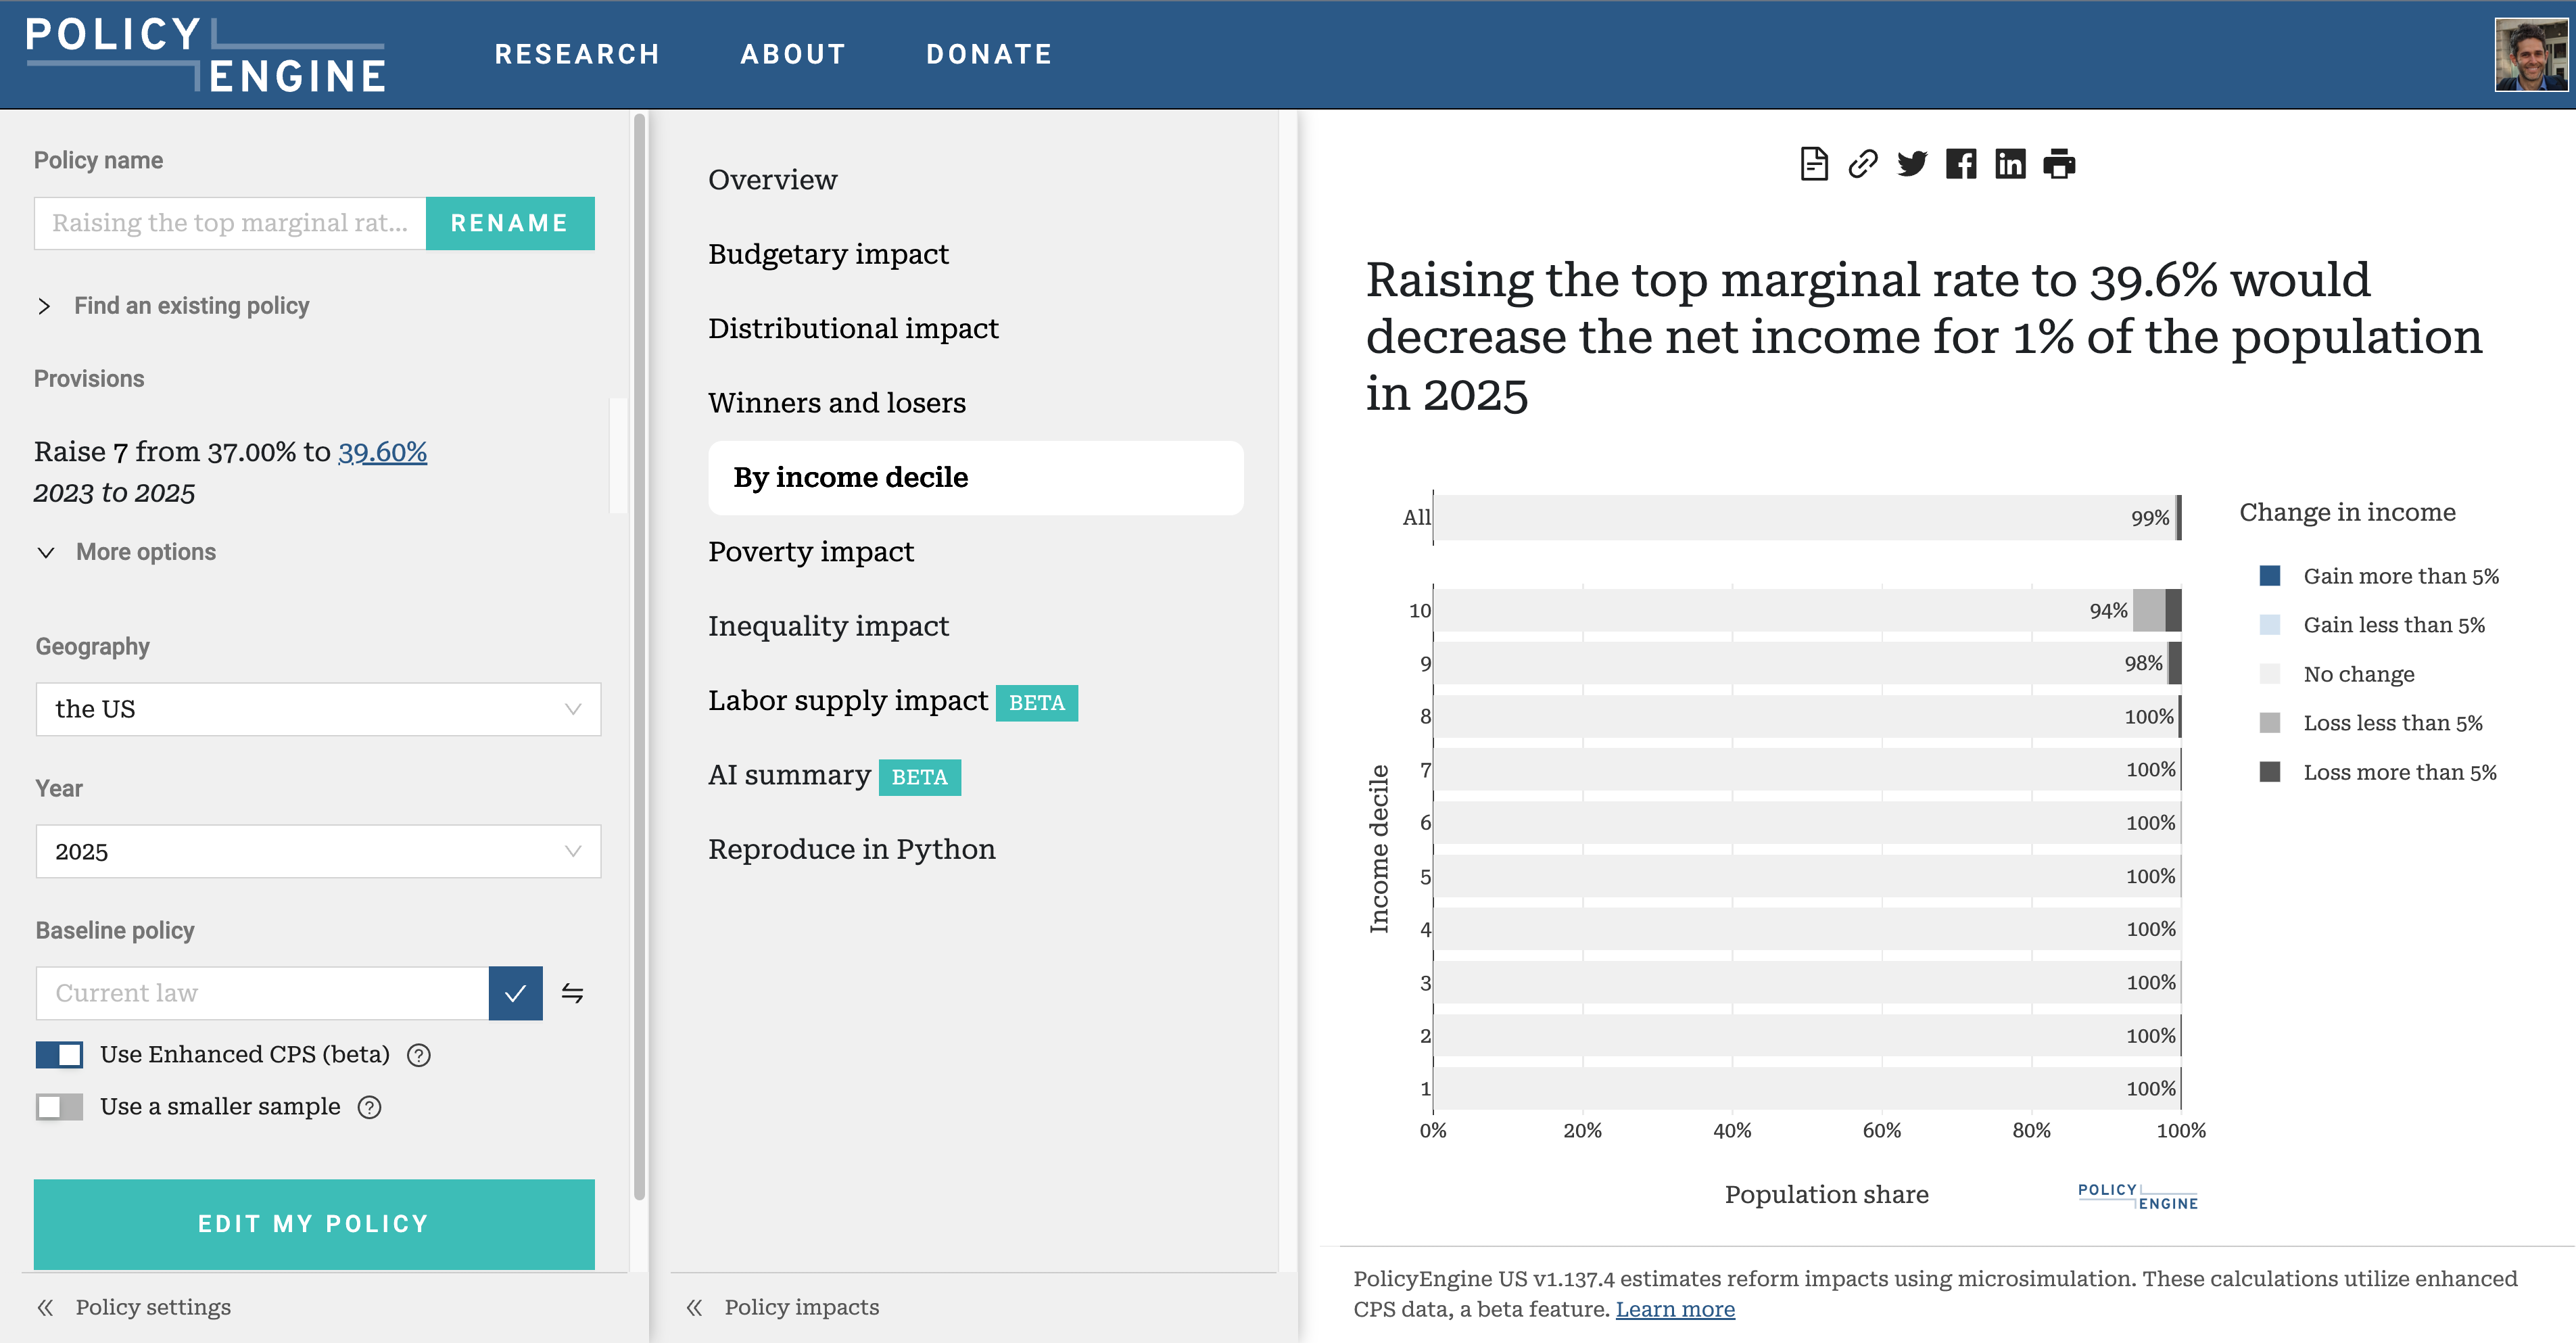
\includegraphics[width=\textwidth]{figures/policyengine_results.png}
    \caption{Example distributional analysis from PolicyEngine showing population impacts by income decile.}
    \label{fig:policyengine_results}
\end{figure}

\subsubsection{Python Package}

The Python package provides programmatic access with just a few lines of code:

\begin{verbatim}
from policyengine_us import Microsimulation

# Load enhanced CPS dataset
sim = Microsimulation(dataset="enhanced_cps_2024")

# Analyze a tax reform
reform = {
    "gov.irs.tax_rate.single": {
        2024: [
            {"threshold": 400_000, "rate": 0.396}
        ]
    }
}
reformed = Microsimulation(reform=reform)

# Calculate revenue impact
baseline_revenue = sim.calculate("income_tax").sum()
reform_revenue = reformed.calculate("income_tax").sum()
revenue_impact = reform_revenue - baseline_revenue

# Analyze impacts by group
income_deciles = sim.calculate("income_decile")
for decile in range(1, 11):
    mask = income_deciles == decile
    impact = reformed.calculate(
        "household_net_income",
        mask=mask
    ).mean() - sim.calculate(
        "household_net_income",
        mask=mask
    ).mean()
    print(f"Decile {decile}: ${impact:,.0f}")
\end{verbatim}

\subsubsection{International Applications}

The same enhancement methodology and software infrastructure powers PolicyEngine UK, which incorporates additional data sources including the Living Costs and Food Survey (for consumption) and Wealth and Assets Survey. This demonstrates the approach's adaptability to different national contexts and data environments.

While designed for seamless integration with PolicyEngine, the enhanced dataset is also available as a standalone HDF5 file that can be used with other microsimulation frameworks, promoting broader research applications while maintaining the benefits of integrated analysis tools.